\section{Test Collection}
\section{Data Curation Error Analysis}
\section{IPC Filter Errors}
\section{Baseline}
\section{Evaluation Metrics}





%In this section, we focus on analysing not retrieved relevant (False Negative (FN)) patents. 
%%\vspace{-2mm} 
%CLEF-IP collection has two main characteristics that leads in two main causes of the error: 
%\begin{enumerate}
%\item \textit{Missing `Description': } Each patent in the collection consisted of multiple versions of documents in XML format labelled as $ A_{1} $, $ A_{2} $ ... $ B_{1} $, and $ B_{2} $. The letter `A' refers to different versions of patent applications. The `B' versions refer to granted patents. We merged different versions of a single patent into one union document as recommended by CLEF-IP%
%\footnote{\texttt{\url{http://www.ifs.tuwien.ac.at/~clef-ip/}}%
%}~\citep{magdy2012toward}. As a result of the merging, some patents in the union collection appears with many missing content fields. Since the `Description' is the longest section in a patent, almost, relevant patent with missing `Description' are not retrieved by the baseline.
%\item \textit{Non-English Patents: } The CLEF-IP has been designed for a multilingual patent search and it consists of patents in three different languages: English, German, and French. All patents have the title in the three languages while just the granted published version of a patent(`B' version) by the EPO should contain the claims section manually translated into all three languages. The description section of all patents is always in the original submission language only. Since the design of the baseline did not consider multilinguality, it can not retrieve relevant but non-English patents.   
%\end{enumerate}
%\noindent Fig.(\ref{fig:datacuration}) shows that, overall, \%37 of errors are due to CLEF-IP collection while \%63 of the errors occurs for full English patent documents.
%%\vspace*{-1ex}
%%\vspace{-3.5mm} 
%\begin{figure}[htpb]
%%\vspace{2.5cm}
%\centering
%\section{•}
%
%
%\begin{subfigure}[htpb]{.5\linewidth}
%\centering
%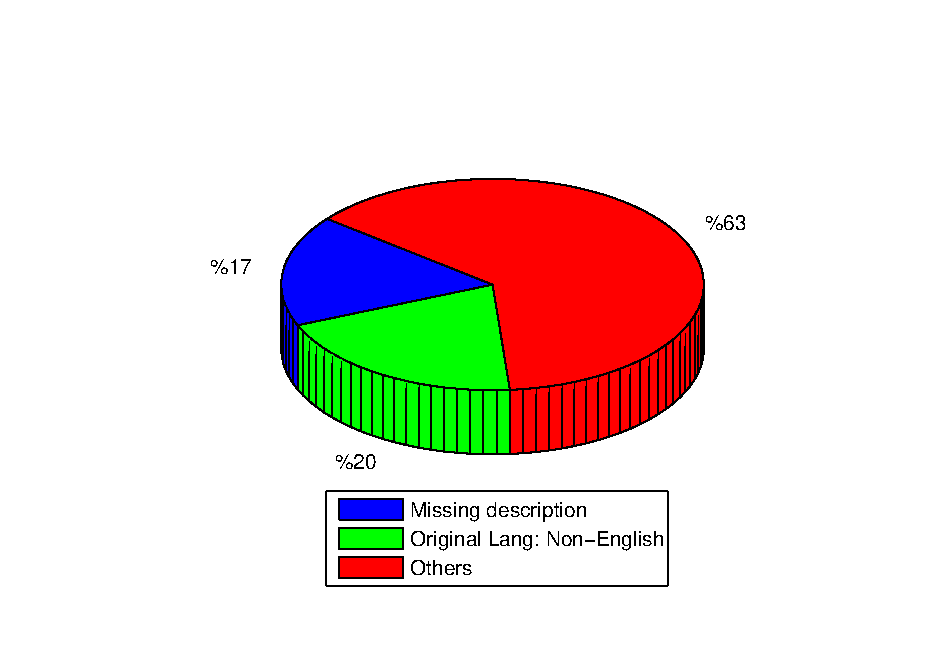
\includegraphics[width=1\textwidth,height=45mm]{figs/analyseFNs100.eps}
%\caption{Cut-off rank(k) = 100}
%\label{fig:datacurationk100}
%\end{subfigure}%\\[1ex]%
%\begin{subfigure}[htpb]{.5\linewidth}
%\centering
%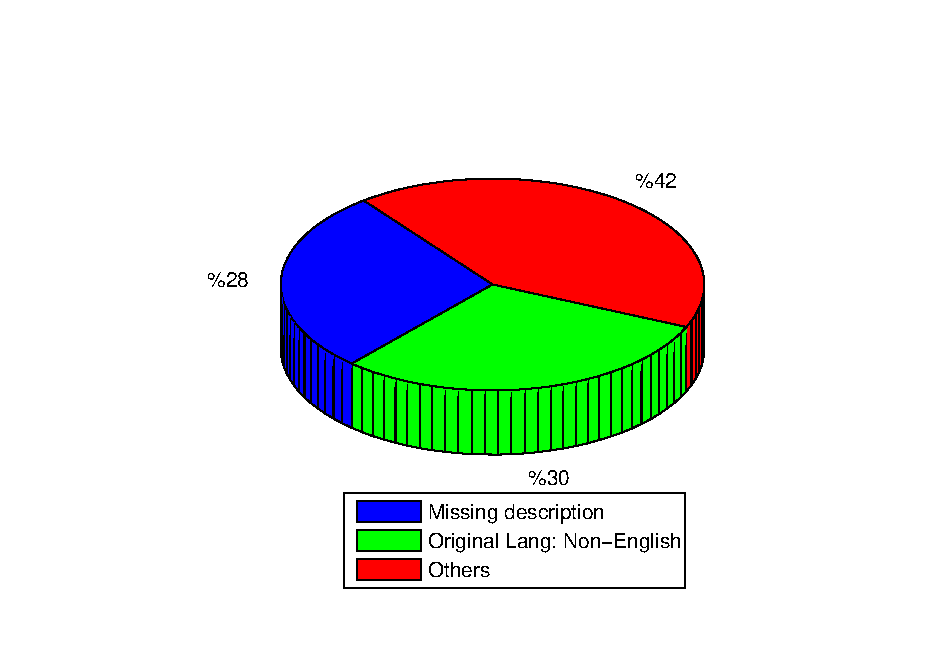
\includegraphics[width=1\textwidth,height=45mm]{figs/analyseFNs1000.eps}
%\caption{Cut-off rank(k) = 1000}
%\label{fig:datacurationk100}
%\end{subfigure}
%\caption{Average percentage of errors due to missing `Description', non-English original language. Overall, \%37 of errors are because of data curation while \%63 of English complete patent documents can not be retrieved. Increasing k from 100 to 1000 reduces the errors of red area, but \%42 is still notable.}
%\label{fig:datacuration}
%\end{figure}
%\FloatBarrier
%%\noindent
%
%%Table \ref{tab:FNs} compares the average percentage of relevant patents which are not retrieved at top 100, 200, and 1000. 
%%\begin{table*}[htpb]
%%  \begin{center}
%%  \input table/FNs.tex  
%%  \caption{The percentage of relevant documents which are not retrieved at top 100, k= 100, over all test queries. In average, \%57 of relevant patents can not be retrieved by the system at top 100.}
%%  \label{tab:FNs}
%%  \end{center}  
%%\end{table*}
%%\FloatBarrier 
%%\noindent
%
%
%%We categorised the source of failure in three groups:
%%\begin{enumerate}
%%\item patents with missing description.
%%\item patents with non-English original language.
%%\item others: patents which are complete and their original language is English. The reason that they are not retrieved is still unknown, but our hypothesis is that these patents can not be retrieved because they have less term overlap with their related query. 
%%%containing the least term overlap with the query.
%%\end{enumerate}
%%The two first groups are the characteristic of our collection and we are not interested in improve the baseline to retrieve them. Whereas, we are interested in improve our system to be able to retrieve the third group.
%%Figure \ref{fig:failingCategory} shows the percentage of each failure source averaged over all queries in FN subset (k = 100).
%%\begin{figure}[htpb]
%%   \centering
%%   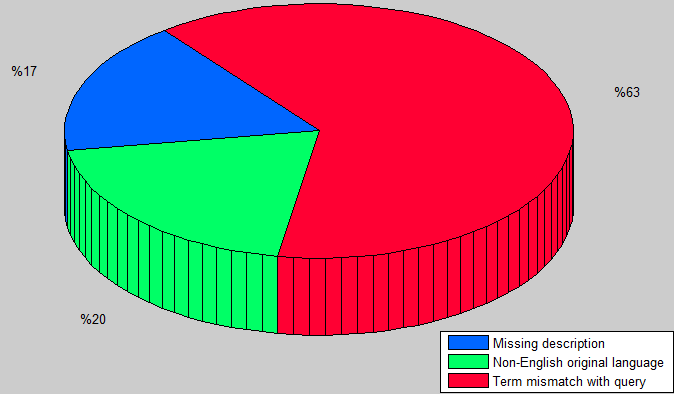
\includegraphics[width=0.55\textwidth,height=45mm]{figs/failingCategory.png}
%%   \caption{Average percentage of patents with missing description, non-English original language, and term mismatch with the query in FN patents over all queries.(k=100).}  
%%   \label{fig:failingCategory} 
%%\end{figure}
%%\FloatBarrier 
%%\noindent
%
%By increasing the ranking threshold to 1000, the percentage of term mismatch failure source decreases in FN subset; Whereas, \%41 is still considerable. 
%
%%\begin{figure}[htpb]
%%   \centering
%%   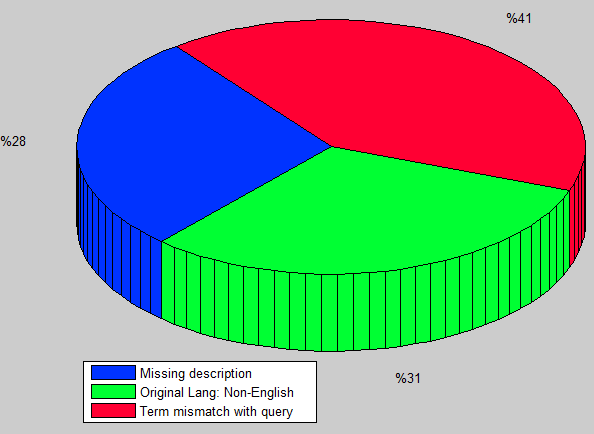
\includegraphics[width=0.55\textwidth,height=55mm]{figs/FNs-k1000.png}
%%   \caption{Average percentage of patents with missing description, non-English original language, and term mismatch with the query in FN patents over all queries.(k=1000).}  
%%   \label{fig:FNs-k1000} 
%%\end{figure}
%%\FloatBarrier 
%%\noindent
%
%We can conclude from Fig. \ref{fig:datacuration} that the main reason, which relevant documents are not retrieved, is the term mismatch between the query and relevant patents,  even in top 1000 documents. The portion of missing description and non-English original language are also high enough to deteriorate the system performance. In our research, we focus on term mismatch between query and relevant documents not missing description or multilinguality which are specific to clef-ip data collection.
%
%Our detailed results also indicate that by increasing the ranking threshold from 100 to 1000, the number of false negatives due to term mismatch between query and relevant documents decreased. Whereas there are some queries that their relevant patents in English do not retrieve even at the rank 1000. 
%
%The focus of this research is to identify the reasons that the system fails to retrieve patents in the red area, where the patents are complete English documents. Hence, in the rest of this paper, we continue our experiment in the red area.\\\\
%\textbf{Anecdotal Examples}\\
%In following experiments, we selected five sample queries from the category: "other"; The following figures show the query term frequency in relevant not-retrieved patents. 
%\begin{landscape}
%\begin{figure}[htpb]
%   \centering
%   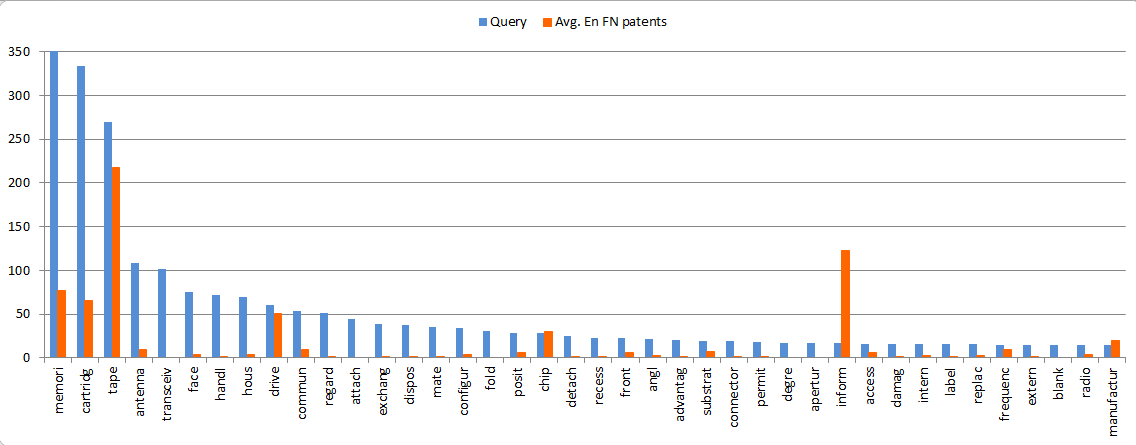
\includegraphics[width=\columnwidth,height=100mm]{figs/pac1035-avgEnFNs.png}
%   \caption{Comparing term frequencies in query, and average term frequencies in relevant not-retrieved patents for Query: PAC-1035. 6/8 patents which are also English can not be retrieved before rank 100, but all can be retrieved before the rank 1000. This indicates that although there is few overlap between query and relevant patents, they will be retrieved but at higher ranks after 100.} 
%   \label{fig:fn-pac1035} 
%\end{figure}
%\end{landscape}
%\FloatBarrier
%\noindent
%  
%\begin{landscape}
%\begin{figure}[htpb]
%   \centering
%   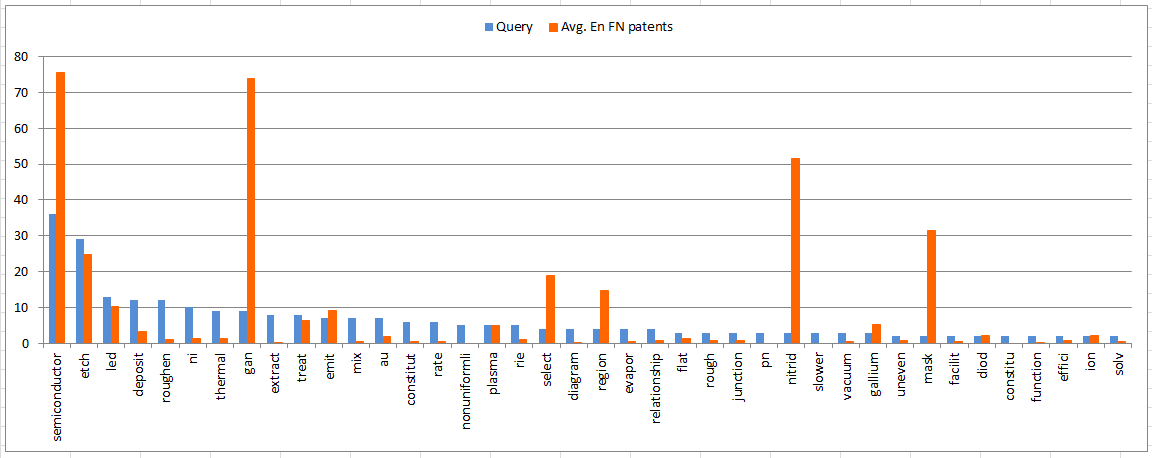
\includegraphics[width=\columnwidth,height=100mm]{figs/fn-pac1142.png}
%   \caption{Comparing term frequencies in query, and average term frequencies in relevant not-retrieved patents for Query: PAC-1142. (En FNs)/FNs = 9/10, @ k=100, and still (En FNs)/FNs = 7/10 @ k=1000. This indicates that 7 relevant patents for this query are not retrievable.} 
%   \label{fig:fn-pac1142} 
%\end{figure}
%\end{landscape}
%\FloatBarrier
%\noindent
%
%\begin{landscape}
%\begin{figure}[htpb]
%   \centering
%   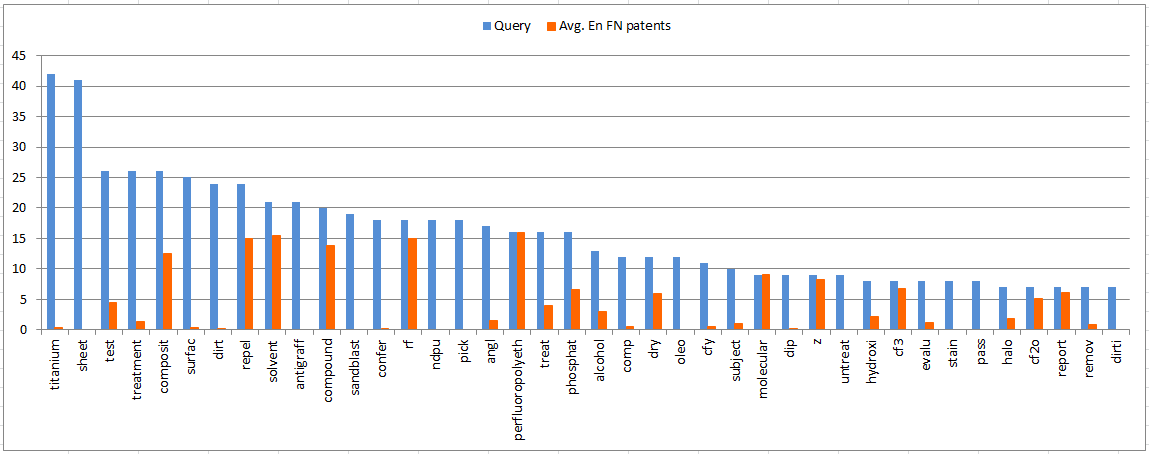
\includegraphics[width=\columnwidth,height=100mm]{figs/fn-pac1216.png}
%   \caption{Comparing term frequencies in query, and average term frequencies in relevant not-retrieved patents for Query: PAC-1216. This query is an example that its English relevant patents (5/6) can not be retrieved even at rank 1000.} 
%   \label{fig:fn-pac1216} 
%\end{figure}
%\end{landscape}
%\FloatBarrier
%\noindent
%
%\begin{landscape}
%\begin{figure}[htpb]
%   \centering
%   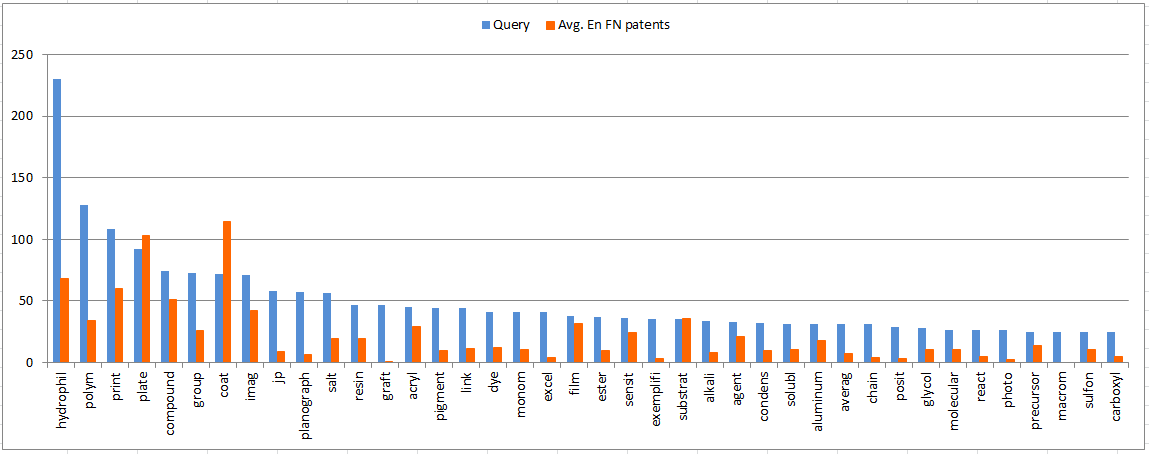
\includegraphics[width=\columnwidth,height=100mm]{figs/fn-pac1379.png}
%   \caption{Comparing term frequencies in query, and average term frequencies in relevant not-retrieved patents for Query: PAC-1379. (En FNs)/FNs = 14/17, @ k=100, and still (En FNs)/FNs = 12/17, @ k=1000. This indicates that 12 English relevant patents for this query are not retrievable.} 
%   \label{fig:fn-pac1379} 
%\end{figure}
%\end{landscape}
%\FloatBarrier
%\noindent
%
%\begin{landscape}
%\begin{figure}[htpb]
%   \centering
%   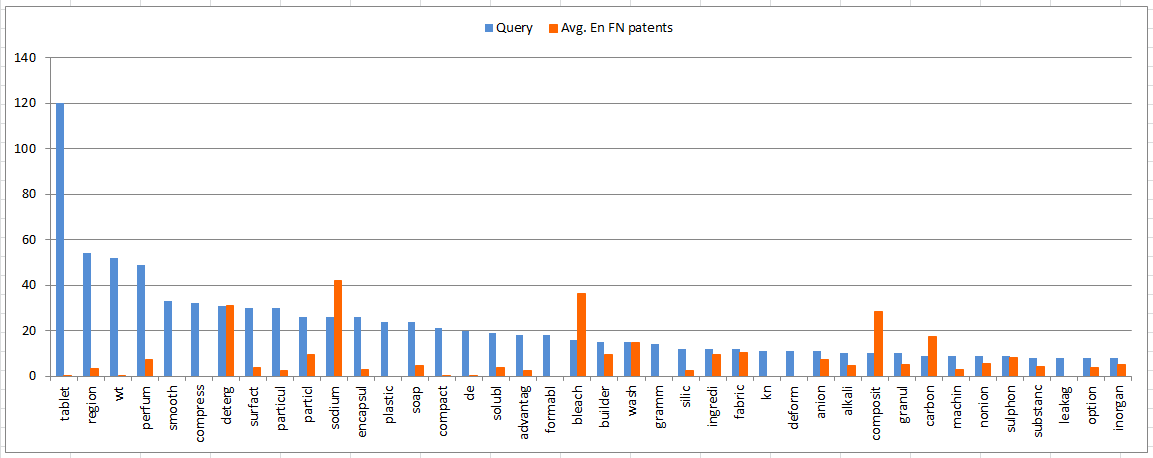
\includegraphics[width=\columnwidth,height=100mm]{figs/fn-pac1604.png}
%   \caption{Comparing term frequencies in query, and average term frequencies in relevant not-retrieved patents for Query: PAC-1604. (En FNs)/FNs = 10/19, @ k=100, and still (En FNs)/FNs = 9/19 @ k=1000. This indicates that 9 English relevant patents for this query are not retrievable.} 
%   \label{fig:fn-pac1604} 
%\end{figure}
%\end{landscape}
%\FloatBarrier
%\noindent
%Our experiments showed the reason that some relevant patents are not retrieved by the system is not that there is zero term overlap between the query and documents, it is low weighting of query terms in the relevant documents. 
%
%
%
%%\begin{table*}[htpb]
%%  \begin{center}
%%  \input table/errorCategory.tex  
%%  \caption{Percentage of missing, non-English, and term mismatch error category in FN patents. }
%%  \label{tab:threshold}
%%  \end{center}  
%%\end{table*}
%%\FloatBarrier 
%%\noindent
%
%%Patent retrieval is a recall-oriented task and it is important to retrieve all relevant patents appear at top of the list. Patent examiners, our users, usually prefer to look at 100-200 top retrieved patents. Table \ref{tab:threshold} shows about \%16 decrease in recall which are not desired for our users. 
%%\begin{table*}[htpb]
%%  \begin{center}
%%  \input table/threshold.tex  
%%  \caption{Comparing performance of the baseline by changing the retrieval threshold.}
%%  \label{tab:threshold}
%%  \end{center}  
%%\end{table*}
%%\FloatBarrier 
%%\noindent
%%
%%\begin{figure}[htpb]
%%   \centering
%%   \includegraphics[width=0.65\textwidth,height=65mm]{figs/a1000.png}
%%   \caption{Baseline performance variation over all queries (k=1000).}  
%%   \label{fig:a1000} 
%%\end{figure}
%%\FloatBarrier 
%%\noindent
%%%
%%%\begin{figure}[htpb]
%%%   \centering
%%%   \includegraphics[width=0.65\textwidth,height=65mm]{figs/a100.png}
%%%   \caption{Baseline performance variation over all queries (k=100).}  
%%%   \label{fig:a100} 
%%%\end{figure}
%%%\FloatBarrier 
%%%\noindent
%%
%%\begin{figure}[htpb]
%%\label{fig:base}
%%        \centering
%%        \begin{subfigure}[b]{0.6\textwidth}
%%        \centering
%%                \includegraphics[width=1\textwidth,height=65mm]{figs/a100.png}
%%                \caption{ }
%%                \label{fig:baseperformancea}
%%        \end{subfigure}%
%%        ~ %add desired spacing between images, e. g. ~, \quad, \qquad, \hfill etc.
%%          %(or a blank line to force the subfigure onto a new line)
%%        \begin{subfigure}[b]{0.6\textwidth}
%%        \centering
%%                \includegraphics[width=1\textwidth,height=65mm]{figs/a1000.png}
%%                \caption{ }
%%                \label{fig:baseperformanceb}
%%        \end{subfigure}
%%       \caption{
%%                Baseline performance variation over all queries (a) k=1000.
%%                (b) k=100.
%%                } 
%%\end{figure}
%%\FloatBarrier
%%\noindent
%%Figure \ref{fig:baseperformancea} and \ref{fig:baseperformanceb} show the variation of the baseline system performance. Figure \ref{fig:baseperformancea} is when choosing the top rank k = 100 and figure \ref{fig:baseperformanceb} is for k = 1000. It can be seen that 'Recall' and 'PRES' skew up when we increase the rank threshold, but there is no significant improvement for 'Average Precision (AP)' because it is more sensitive to finding relevant documents at very high ranks regardless of the number of documents to be checked by the user. However, 'PRES' is more sensitive to the average ranking of the relevant retrieved documents as a whole relative to the maximum number of documents the user is willing to check. Foe example, when Nmax=1000, the ranks {32, 35, 46} are considered relatively good compared to this number. Nevertheless, when calculating PRES with Nmax=100, the PRES value will be less which represents the average ranking of the relevant documents relative to the maximum number of documents to be checked. Low 'AP' indicates that system is also incapable of retrieving patents at top of the list with high ranks. The reason was indicated in previous section (term level analysis), irrelevant patents have more common words with the query which ends in retrieving them at top of the list. The solution is finding the noisy words which appear more in the irrelevant documents and should be identified and removed. 
%%%\begin{list}{-}{}
%%%\end{list}
%%
